\subsection{Mix it up}
\frame
{
  \frametitle{Pros and Cons}

  \begin{itemize}
  \item<1-> Testing story
  \item<2-> Provisioning
  \item<3-> React to changes
  \item<4-> Ruby vs Python
  \end{itemize}
}

\frame
{
  \frametitle{Pros and Cons}

  \begin{itemize}
  \item<1-> Chef ~60 builtin resources
  \item<2-> SaltStack ~330 builtin modules
  \item<3-> Chef Community Cookbooks
  \item<4-> SaltStack zipped modules
  \item<5-> Write your own recipe/module
  \end{itemize}
}

\frame
{
  \frametitle{Why the mix?}
  \begin{center}
    Why mix Chef and SaltStack?
  \end{center}
}

\frame
{
  \frametitle{Why the mix?}

  \begin{itemize}
  \item<1-> Instant remote execution
  \item<2-> \textit{knife ssh 'chef\_environment:staging' 'echo foobar'}
  \begin{itemize}
    \item<3-> Doesn't scale well
    \item<4-> Requires ssh access
    \item<5-> Ssh using user or root?
  \end{itemize}
  \item<6-> Chef Push Jobs?
  \end{itemize}
}

\subsection{Instant Alternatives}
\frame
{
  \frametitle{Chef Push Jobs}
  \begin{center}
    The pushy Chef
  \end{center}
}

\frame
{
  \frametitle{Chef Push Jobs}
  \begin{center}%
    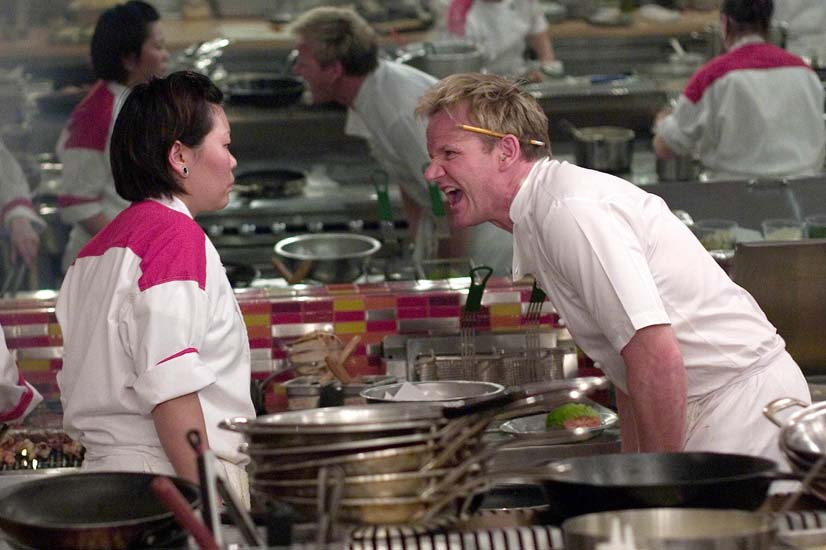
\includegraphics[height=5cm]{images/pushy_chef.jpg}
  \end{center}%
}

\frame
{
  \frametitle{Chef Push Jobs}

  \begin{itemize}
  \item<1-> Separate Cookbook
  \item<2-> Two new ports (10000 and 10003) on Chef Server
  \item<3-> Needs a plugin on the Chef Server
  \item<4-> Uses ZeroMQ
  \item<5-> Doesn't feel as elegant as Salt
  \end{itemize}
}

\subsection{Both sides are open}
\frame
{
  \begin{center}
    Both sides are open
  \end{center}
}

\frame
{
  \frametitle{Mix and match}

  \begin{itemize}
  \item<1-> salt.modules.chef
  \item<2-> https://supermarket.chef.io/cookbooks/salt
  \item<3-> Transition phase
  \item<4-> Test Kitchen vs Python Unit Tests
  \end{itemize}
}
